\def\year{2015}
%File: formatting-instruction.tex
\documentclass[letterpaper]{article}
\usepackage{aaai}
\usepackage{times}
\usepackage{helvet}
\usepackage{courier}

\usepackage{graphicx}
\usepackage{subfigure}
\usepackage{amssymb}
\usepackage{amsmath}
\usepackage{algorithm}
\usepackage{algorithmic}
\usepackage{amsthm}

\newtheorem{lem}{Lemma}
\newtheorem{thm}{Theorem}
\newtheorem{prop}{Proposition}
\theoremstyle{remark}
\newtheorem*{rem}{Remark}
\theoremstyle{definition}
\newtheorem{defn}{Definition}

\renewcommand{\algorithmicrequire}{\textbf{Input:}}
\renewcommand{\algorithmicensure}{\textbf{Initialize:}}
%\newcommand{\vector}{\mathbf}
\DeclareMathOperator{\sign}{sign}

\frenchspacing
\setlength{\pdfpagewidth}{8.5in}
\setlength{\pdfpageheight}{11in}
\pdfinfo{
/Title (Online Transfer Learning with Heterogeneous Source)
/Author (Author1, Author2, Author3)
/Keywords (Transfer Learning, Heterogeneous Transfer, Online Learning)
}
\setcounter{secnumdepth}{0}  
 \begin{document}
% The file aaai.sty is the style file for AAAI Press 
% proceedings, working notes, and technical reports.
%
\title{Online Transfer Learning with Heterogeneous Source}
\author{Author1\\ Address line\\
\And Author2 \\ Address line\\
\And Author3 \\ Address line\\
}
\maketitle
\begin{abstract}
%\begin{quote}
Heterogeneous transfer learning aims to build the model in the target domain by leveraging knowledge extracted from other heterogeneous source domains.
In this paper, we investigate online heterogeneous transfer learning problem, which considers a classification on the target domain in an online fasion.
The motivation of our work is to utilize data in the heterogeneous source domain to promote the ability of classifier.
The challenges in online heterogeneous transfer learning mainly come from two aspects.
The first one is that the feature spaces of the source and target domains are completely different, which leads to the difficulty for knowledge transfer.
The second one is that we do not have enough prior training data from the target domain to build a precise relationship across the source and target domains.
With regard to aforementioned problems, we propose effective algorithms based on ensemble strategy.
We first construct a connection between the source and target domains using co-occurrence data, and then build a weighted $K$ nearest neighbor classifier based on the heterogeneous data.
Combining with the hypothesis trained on the target domain, we obtain the final classifier.
We also theoretically analyze the mistake bound of our proposed algorithms under the $\mathbf{Hedge(\beta)}$ framework.
The experiments are conducted for image classification by exploiting the knowledge learnt from the text data.
Encouraging results demonstrate the effectiveness of our algorithms.

%\end{quote}
\end{abstract}


\section{Introduction}

Transfer learning \cite{pan2010survey}, which devotes to transferring knowledge extracted from the source domain to the target domain, has been actively studied in recent years.
According to the relationship between the source and target domains, we can categorize transfer learning into two groups: homogeneous transfer and heterogeneous transfer.
A great number of works in the last decade successfully deal with homogeneous transfer learning problem \cite{liao2005logistic,dai2007boosting,dai2007transferring,eaton2011selective}, which assumes that the data spaces of the source and target domains are the same.
Nevertheless, more and more studies consider heterogeneous transfer learning problem.
Heterogeneous transfer considers the situation that either the feature spaces or the output spaces of the source and target domains are different.

Most works regarding heterogeneous transfer address an offline learning problem.
In this paper, we investigate online heterogeneous transfer learning problem, whose test data instances arrive sequentially.
Our motivation is to achieve better performance on a classification task in the target domain using knowledge learnt from the data in the heterogeneous source domain.
There are two principal challenges in online heterogeneous transfer problem.
The first one is the fact that feature spaces of the source and target domains are completely different, which makes it difficult to construct relationship across domains.
The second one comes from the characteristic of online learning problem.
As the data instances arrive in an sequential manner, we do not have enough training data from the target domain in advance.
Thus, we cannot adopt a training method to build precise relasionship between the source and target domains.

In order to solve aforementioned problems, we propose \textbf{O}nline \textbf{H}eterogeneous \textbf{T}ransfer (OHT) algorithms based on $\mathbf{Hedge(\beta)}$ framework.
Firstly, by calculating the similarity between the test instance and the heterogeneous data instance using co-occurrence data, we construct a connection across the domains.
Next, we adopt weighted $K$ nearest neighbor algorithm to obtain hypothesis in the heterogeneous source domain.
At the same time, a traditional online learning algorithm is applied in the target domain to produce another hypothesis.
Combining two hypotheses based on $\mathbf{Hedge(\beta)}$ framework, we get the final classifier.
We also analyze the theoretical bound of our proposed algorithms.

The experiments are conducted for image classification by taking advantage of knowledge in the text data.
We make use of NUS-WIDE dataset to generate binary classification tasks.
Empirical results show that our algorithms outperform the baseline methods.

\section{Related Work}

The topics that our work is related to are heterogeneous transfer learning and online learning.
In this section, we review some related works and address the differences between our work and the existing works.

\subsection{Heterogeneous Transfer Learning}
The objective of heterogeneous transfer learning is to solve a problem in the target domain by leveraging knowledge extracted from other heterogeneous source domains with different feature space.
\cite{wei2011heterogeneous} applied restricted Boltzmann machine to perform heterogeneous transfer learning task.
And depp learning technique is introduced into heterogeneous transfer problem in \cite{zhou2014hybrid}.
There are also some existing works studying heterogeneous transfer learning problem using co-occurrence data.
\cite{yang2009heterogeneous} leverage text data for image clustering, and \cite{zhu2011heterogeneous} utilize text data for image classification task.
\cite{wang2009building} proposed a algorithm to build two separate classifiers based on text features and image features, and then the final classifier are trained to combine them.
And \cite{ng2012co,wu2014co,tan2014mixed} constructs transition probabilities based on co-occurrence information among instances from different domains, and applied random walker method to deal with classification task.

However, above-mentioned studies require training data in the source and target domains.
\cite{zhu2011heterogeneous} utilize training data to learn high-level features which help to construct extra representation for target images.
And the transition probabilities matrix used in \cite{ng2012co,wu2014co} also need prior training data in the source as well as target domains.
Since all the data instance in the target domain arrive sequentially, we do not have enough data for training process.
To deal with this problem, we establish a relationship based on the similarity between the instance in the target domain and the heterogeneous data without a batch training procedure.

\subsection{Online Learning}

Online learning has been actively studied for years.
Compared to the off-line machine learning problem that training data are given first, online learning learner receives data instances sequentially.
An online learning learner make a prediction immediately and adjust itself during the process of task.
One of the classic algorithms of online learning is Perceptron algorithm \cite{rosenblatt1958perceptron}, which move the decision bound towards the direction of an instance which is labeled wrong.
Passive-Aggressive algorithm and its variants take the criterion of maximum margin into account \cite{crammer2006online}.

However, only a few works address transfer learning in an online fasion.
\cite{zhao2010otl,zhao2014online} adopt an ensemble strategy to deal with the homogeneous transfer learning problem, and a co-regularization principle is used to handle the heterogeneous transfer learning problem.
Nevertheless, the multi-view approach for online heterogeneous transfer in \cite{zhao2010otl,zhao2014online} assume that the feature space of the source domain is a subset of that of the target domain.
Instead, we consider a situation that the feature spaces of the source and target domains do not share any common subset.
Co-occurrence data are used to help us transfer knowledge learnt from the heterogeneous source domain.

\section{Problem Definition}

Suppose that we are given some instances $\{\mathbf{x}_{i}^{s}, y_{i}^{s}\}$ in the source data space $\mathcal{X}^{s} \times \mathcal{Y}^{s}$, where $\mathcal{X}^{s} = \mathbb{R}^{d^s}$ and $\mathcal{Y}^{s} = \{+1,-1\}$.
The objective of online transfer learning is to learn a classifier $f(\mathbf{x}_{t})$ to classify the instance on a target domain in a online fasion.
The data space of the target domain is $\mathcal{X} \times \mathcal{Y}$, where $\mathcal{X} = \mathbb{R}^{d}$ and $\mathcal{Y} = \{+1,-1\}$.
Specifically, the task of online heterogeneous transfer learning is a sequential process, during which an image instance $\mathbf{x}_t$ comes at the $t$-th trial, and the classifier generates a predicted class label $\hat{y}_{t}$.
Then the classifier receives the true class label $y_t$ and update itself to obtain better classification ability.

In our problem setting, $\mathcal{Y} = \mathcal{Y}^{s}$, which means the same class label in two domains indicates the same class, for instance, $+1$ indicates an instance labeled vehicle and $-1$ indicates an instance labeled tree.
Nevertheless, the motivation of us is to conduct online classification task by leveraging knowledge in a heterogeneous source domain.
Formally, $\mathcal{X} \cap \mathcal{X}^{s} = \varnothing$.
We cannot directly transfer information from a completely different source domain.
Therefore, a sophistecated knowledge transfer method is proposed.

\section{Methods}

In this section, we describe the details of our proposed algorithms.
We extend HomOTL algorithms, which exploit knowledge in a homogeneous source domain, to tackle the online heterogeneous transfer learning problem.
We first introduce our approach of how to establish relationship between two different domains to build classifier using heterogeneous source data.
Then we present online heterogeneous transfer learning algorithms.

\subsection{Heterogeneous Knowledge Transfer}

In order to transfer knowledge in the heterogneous source to the target domain, we construct a connection between two domains, and then design a hypothesis to predict class label of the instance in the target domain.

Our idea is to bridge two domains via their co-occurrence information.
Given some co-occurrence data instances $\{ \mathbf{x}_{i}^{o} \}$ in the data space $\mathcal{X}^o$, which can be split into two part $\mathcal{X}^{(1)}$ and $\mathcal{X}^{(2)}$.
Then we have $ \mathbf{x}_{i}^{o} = (\mathbf{x}_{i}^{(1)}, \mathbf{x}_{i}^{(2)}) $.
The first part of the feature space of co-occurrence data is the same as the feature space of the target domain, and the second part is the same as the feature space of the source domain.
More specifically, we have $\mathcal{X}^{(1)} = \mathcal{X}$, and $\mathcal{X}^{(2)} = \mathcal{X}^s$.

It is convenience to collect co-occurrence data from the Internet.
For example, tagged images from Flickr can be used as the co-occurrence data between image data space and text data space.
When $\mathcal{X}$ is the feature space of English document and $\mathcal{X}^s$ is the feature space of Chinese document, the co-occurrence data can be collected from Wikipedia webpages titled by corresponding term.
Figure illustrates the relationship among two domains and the co-occurrence data.

As $\mathcal{X}^{(1)} = \mathcal{X}$, at $t$-th trial, we can construct a similarity vector $Sim_{t}^{(1)}$ to measure the affinity between $\mathbf{x}_t$ and each instance of co-occurrence data. 
The $i$-th element $Sim_{t}^{(1)}(i)$ is Pearson correlation between $\mathbf{x}_t$ and $\mathbf{x}_{i}^{o}$.
The formula shows as follows:
$$ Sim_{t}^{(1)}(i) = \frac{(\mathbf{x}_t - \bar{\mathbf{x}}_t) \cdot (\mathbf{x}_{i}^{(1)} - \bar{\mathbf{x}}_{i}^{(1)})}{\| \mathbf{x}_t - \bar{\mathbf{x}}_t \| \| \mathbf{x}_{i}^{(1)} - \bar{\mathbf{x}}_{i}^{(1)} \|} $$
where $\bar{\mathbf{z}} = mean(\mathbf{z})$.
Also, we can construct a similarity matrix $Sim^{(2)}$ to measure the affinity among instances from co-occurrence data and the heterogeneous source domain.
The formula of the $(i,j)$-th element $Sim^{(2)}(i,j)$ is
$$ Sim^{(2)}(i,j) = \frac{(\mathbf{x}_{i}^{(2)} - \bar{\mathbf{x}}_{i}^{(2)}) \cdot (\mathbf{x}_{j}^{s} - \bar{\mathbf{x}}_{j}^{s})}{\| \mathbf{x}_{i}^{(2)} - \bar{\mathbf{x}}_{i}^{(2)} \| \| \mathbf{x}_{j}^{s} - \bar{\mathbf{x}}_{j}^{s} \|} $$
Finally, we obtain a similarity vector $Sim_t$ between $\mathbf{x}_t$ and each instance in the heterogeneous source domain, with its $j$-th entry is calculated by 
$$ Sim_t(j) = \sum\limits_i Sim_{t}^{(1)}(i) Sim^{(2)}(i,j) $$

Based on $Sim_t$, we predict the class label of instance $\mathbf{x}_t$ by weighted $K$ nearest neighbor classifier:
$$ h_{t}^{s}(\mathbf{x}_t) = \sum\limits_{i \in N} \frac{Sim_t(i)}{\sum\limits_{i \in N} Sim_t(i)} y_i $$
where $N$ is the set of identifiers of $K$ nearest neighbors in the heterogeneous source domain.

\subsection{Online Heterogeneous Transfer Algorithms}

Given a hypothesis obtained from the hetegeneous source domain, we can utilize the ensemble learning stragety similar to HomOTL algorithms.

We first construct a prediction function in the target domain using online learning algorithm PA, and then combine two hypotheses to get final classifier.
According to the loss value suffered by each hypothesis seperately, we dynamically update two weights of both hypotheses.
Without loss of generality, we use linear function in the target domain to simplify the description.
Through the kernel trick, we are able to tackle the non-linear classification problem.

Algorithm 1 presents the process of the proposed online heterogeneous transfer learning algorithm 1 (OHT1).
$w_{1}^{s}$ and $w_1$ reflect the prior confidence we have on two hypotheses, and must sum to 1.
If we have no preference on any of them, we can simply set $w_{1}^{s} = w_{t} = \frac{1}{2}$, which is also the setting we used in our experiments.
Function $\varOmega(z) = \max \{ 0, \min \{ 1, \frac{z+1}{2} \}\}$ projects $z \in \mathbb{R}$ to range $[0,1]$.
In order to adjust two weights dynamically, exponentially weighting update method \cite{cesa2006prediction} is used.

It is worthwhile to note that the equation in step 8, which calculate the updating factor of linear classifier trained on the target domain, can be replaced by two variants.
In \cite{crammer2006online}, PA-\uppercase\expandafter{\romannumeral1} introduces a non-negative linear slack variable into PA, and PA-\uppercase\expandafter{\romannumeral2} introduces a quadratic slack variable.
The corresponding equations of calculation of $\tau$ are $\tau_t = \min \{ C, \frac{\ell_{t}^{*}}{{\|\mathbf{x}_t\|}^2} \} $ and $ \tau_t = \frac{\ell_{t}^{*}}{{\|\mathbf{x}_t\|}^2 + \frac{1}{2C}} $ respectively.
Likewise, by replacing the equation in Step 8, we can obtain two variants OHT1-\uppercase\expandafter{\romannumeral1} and OHT1-\uppercase\expandafter{\romannumeral2}.

\begin{algorithm}
\begin{algorithmic}[1]
\caption{Online Heterogeneous Transfer Algorithm 1 (OHT1)}
\REQUIRE ~~
aggressiveness parameter $C>0$\\ 
%~~~~~~~~~discount parameter $\beta \in (0,1)$\\ 
~~~~~~~~~$\eta = \frac{1}{2}$ \\
~~~~~~~~~heterogeneous source data
\ENSURE ~~
$\mathbf{v} = \mathbf{0}$, $w_{1}^{s} \in (0,1)$, $w_{1} \in (0,1)$, where $w_{1}^{s} + w_1 = 1$
\FOR{$t=1$ to $T$}
\STATE 
  receive instance: $\mathbf{x}_t \in \mathcal{X}$
\STATE
  normalize: $\theta_{t}^{s} = \frac{w_{t}^{s}}{w_{t}^{s}+w_t}, \theta_{t} = \frac{w_{t}}{w_{t}^{s}+w_t}$
\STATE
  predict: $\hat{y}_t = \sign \big( \theta_{t}^{s} \varOmega (h_{t}^{s}(\mathbf{x}_t)) + \theta_{t} \varOmega (\mathbf{v}_t \cdot \mathbf{x}_t) - \frac{1}{2} \big)$
\STATE
  receive correct label: $y_t \in \mathcal{Y}$
\STATE
  compute: 
    $$w_{t+1}^{s} = w_{t}^{s} \exp \big\{ -\eta \big(\varOmega(h_{t}^{s}(\mathbf{x}_t)) - \varOmega(y_t)\big)^2 \big\} $$
    $$w_{t+1} = w_{t} \exp \big\{ -\eta \big(\varOmega(\mathbf{v}_t \cdot \mathbf{x}_t) - \varOmega(y_t)\big)^2 \big\} $$
\STATE
  suffer loss: $\ell_{t}^{*} = \max \{0, 1-y_t(\mathbf{v}_t \cdot \mathbf{x}_t)\}$
\STATE
  set: $\tau_t = \frac{\ell_{t}^{*}}{{\|\mathbf{x}_t\|}^2}$
\STATE
  update: $ \mathbf{v}_{t+1} = \mathbf{v}_t + \tau_t y_t \mathbf{x}_t $
\ENDFOR
\end{algorithmic}
\end{algorithm}

Algorithm 2 summarizes the online heterogeneous transfer learning 2 (OHT2).
OHT2 has a more polarized attitude to two hypotheses.
Indication function $I(\cdot)$ represents whether the hypothesis makes a wrong prediction or not.
The mistake made by a hypothesis will decrease its weight in the next trial.

Similar to OHT1 algorithms, we also have two variants OHT2-\uppercase\expandafter{\romannumeral1} and OHT2-\uppercase\expandafter{\romannumeral2}.

\begin{algorithm}
\begin{algorithmic}[1]
\caption{Online Heterogeneous Transfer Algorithm 2 (OHT2)}
\REQUIRE ~~
aggressiveness parameter $C>0$\\ 
~~~~~~~~~discount parameter $\alpha \in (0,1)$\\ 
~~~~~~~~~heterogeneous source data 
\ENSURE ~~
$\mathbf{v} = \mathbf{0}$, $w_{1}^{s} \in (0,1)$, $w_{1} \in (0,1)$, where $w_{1}^{s} + w_1 = 1$
\FOR{$t=1$ to $T$}
\STATE 
  receive instance: $\mathbf{x}_t \in \mathcal{X}$
\STATE
  normalize: $\theta_{t}^{s} = \frac{w_{t}^{s}}{w_{t}^{s}+w_t}, \theta_{t} = \frac{w_{t}}{w_{t}^{s}+w_t}$
\STATE
  predict: $\hat{y}_t = \sign \big( \theta_{t}^{s} \sign (h_{t}^{s}(\mathbf{x}_t)) + \theta_{t} \sign (\mathbf{v}_t \cdot \mathbf{x}_t) \big)$
\STATE
  receive correct label: $y_t \in \mathcal{Y}$
\STATE
  compute: 
    $$w_{t+1}^{s} = w_{t+1}^{s} \alpha ^ {I(y_t h_{t}^{s}(\mathbf{x}_t) \leq 0)}  $$
    $$w_{t+1} = w_{t+1} \alpha ^ {I(y_t (\mathbf{v}_t \cdot \mathbf{x}_t) \leq 0)}  $$
\STATE
  suffer loss: $\ell_{t}^{*} = \max \{0, 1-y_t(\mathbf{v}_t \cdot \mathbf{x}_t)\}$
\STATE
  set: $\tau_t = \frac{\ell_{t}^{*}}{{\|\mathbf{x}_t\|}^2}$
\STATE
  update: $ \mathbf{v}_{t+1} = \mathbf{v}_t + \tau_t y_t \mathbf{x}_t $
\ENDFOR
\end{algorithmic}
\end{algorithm}


\section{Theoretical Analysis of OHT Algorithms}
In this section, we utilize $\mathbf{Hedge}(\beta)$ algorithm framework to help us understand OHT algorithms.
We also derive mistake bound of OHT algorithms.

At $t$-th trial of online learning problem, $\mathbf{Hedge}(\beta)$ algorithm framework synthesize opinions from different experts based on a weight vector $\mathbf{weight}_t$.
After the loss value of each expert has been received, the weight vector is updated using rule
$$ weight_{t+1}^{i} = weight_{t}^{i} \cdot \beta^{loss_{t}^{i}} $$
where $\beta \in [0,1]$ and $loss_{t}^{i} \in [0,1]$.

In our proposed OHT algorithms, we refer to two hypotheses from two domains as the experts.
We denote the loss value at $t$-th trial of the source domain and the targe domain by $\ell_{t}^{s}$ and $\ell_t$ respectively.
For OHT1 algorithms, we take $\ell_{t}^{s} = (\varOmega(h_{t}^{s}(\mathbf{x}_t)) - \varOmega(y_t)) ^ 2$, $\ell_t = (\varOmega(\mathbf{v}_t \cdot \mathbf{x}_t) - \varOmega(y_t)) ^ 2$, and $\beta = \exp\{-\eta\}$ where $\eta > 0$.
For OHT2 algorithms we take $\ell_{t}^{s} = I(y_t h_{t}^{s}(\mathbf{x}_t) \leq 0)$, $\ell_t = I(y_t (\mathbf{v}_t \cdot \mathbf{x}_t) \leq 0)$, and $\beta = \alpha$.
It is easy to validate that the weight updating strategies in OHT algorithms obey the rule of $\mathbf{Hedge}(\beta)$ algorithm framework.

Notice that loss value $\ell_{t}^{*}$ in step 7 of OHT algorithms is calculated based on the hypothesis trained in the target domain independently.
Specifically, the calculation of $\ell_{t}^{*}$, which comes from PA algorithm, aims to update the hypothesis in the target domain.
However, we use $\ell_{t}^{s}$ and $\ell_t$ to represent the loss suffered by each hypothesis seperately, and adjust the weights of two hypotheses from different domains.

Before we present the mistake bound of our two OHT algorithms, we first give a proposition which can be used to derive mistake bound of both OHT algorithms.

\begin{prop}
%Let $\mathbf{L}_t = (\ell_{t}^{s}, \ell_{t})$ be the loss vector at $t$-th trial, and $\mathbf{W}_t = (\mathbf{w}_{t}^{s}, \mathbf{w}_{t})$ be the weight vector at $t$-th trial.
Given loss $\ell_{t}^{s} \in [0,1]$, $\ell_t \in [0,1]$ and decay factor $\beta \in (0,1)$, for any sequence of loss vectors $\{ (\ell_{t}^{s}, \ell_{t}) | t = 1, 2, \cdots T \} $, we have
$$ \sum\limits_{t=1}^{T} ( \theta_{t}^{s} \ell_{t}^{s} + \theta_t \ell_t ) \leq \frac{1}{1-\beta} \min \big( \varDelta^s, \varDelta \big) $$
where
$ \varDelta^s = \ln(\frac{1}{w_{1}^{s}}) + (\ln \frac{1}{\beta}) \sum\limits_{t=1}^{T} \ell_{t}^{s} $ and $ \varDelta = \ln(\frac{1}{w_{1}}) + (\ln \frac{1}{\beta}) \sum\limits_{t=1}^{T} \ell_{t} $
%\begin{gather*}
%\varDelta^s = \ln(\frac{1}{w_{1}^{s}}) + (\ln \frac{1}{\beta}) \sum\limits_{t=1}^{T} \ell_{t}^{s} \\
%\varDelta = \ln(\frac{1}{w_{1}}) + (\ln \frac{1}{\beta}) \sum\limits_{t=1}^{T} \ell_{t} 
%\end{gather*}
%\begin{equation*}
%\begin{split}
 %\sum\limits_{t=1}^{T} ( w_{t}^{s} \ell_{t}^{s} + w_t \ell_t ) \leq \frac{1}{1-\beta} \min 
 %& \big(\ln(\frac{1}{w_{1}^{s}}) + (\ln \frac{1}{\beta}) \sum\limits_{t=1}^{T} \ell_{t}^{s}, \\
 %& \ln(\frac{1}{w_{1}}) + (\ln \frac{1}{\beta}) \sum\limits_{t=1}^{T} \ell_{t}  \big) 
%\end{split}
%\end{equation*}
\end{prop}

The technique of the proof can be found in \cite{freund1995decision}.
\begin{rem}
The physical meaning of the Proposition 1 is that the entire loss value, which sums up the combined loss at every trial, is not much larger than the loss value maded by the better hypothesis.
At the right side of the inequation, $\ln(\frac{1}{w_{1}^{s}})$ and $\ln(\frac{1}{w_1})$ measure the prior confidence we have on two hypotheses.
If we have no reason to prefer any of them, we simply set $w_{1}^{s} = w_1 = \frac{1}{2}$.
Thus, the upper bound is only depend on the summation of loss made by two hypotheses seperately.
On the other hand, if we accidently trust the right expert, we could get a tighter bound.
For instance, if we choose to believe that $\sum\limits_{t=1}^{T} \ell_{t} < \sum\limits_{t=1}^{T} \ell_{t}^{s}$, and fortunately it is the truth at the same time, then we set $w_1 > w_{1}^{s}$.
Consequently, we get a better bound than the one when we set $w_{1}^{s} = w_{1}$.

Based on Proposition 1, we can analyze the mistake bound of proposed algorithms.

\end{rem}

\subsection{Mistake Bound of OHT1}

In OHT1 algorithms, $\ell_{t}^{s} = (\varOmega(h_{t}^{s}(\mathbf{x}_t)) - \varOmega(y_t)) ^ 2$, $\ell_t = (\varOmega(\mathbf{v}_t \cdot \mathbf{x}_t) - \varOmega(y_t)) ^ 2$, and $\beta = \exp\{-\eta\}$ where $\eta > 0$.
According to Proposition 1, we derive the mistake bound of OHT1 as follows.

\begin{thm}
Let $M$ be the number of mistakes made by OHT1 algorithm, then we have 
$$ M \leq \frac{4}{1-\beta} \min (\varDelta^s, \varDelta) $$
where
$ \varDelta^s = \ln(\frac{1}{w_{1}^{s}}) + (\ln \frac{1}{\beta}) \sum\limits_{t=1}^{T} \ell_{t}^{s} $ and $ \varDelta = \ln(\frac{1}{w_{1}}) + (\ln \frac{1}{\beta}) \sum\limits_{t=1}^{T} \ell_{t} $.
%\begin{equation*}
%\begin{split}
 %M \leq \frac{4}{1-\beta} \min 
 %& \big( \ln(\frac{1}{w_{1}^{s}}) + (\ln \frac{1}{\beta}) \sum\limits_{t=1}^{T} \ell_{t}^{s}, \\
 %& \ln(\frac{1}{w_{1}}) + (\ln \frac{1}{\beta}) \sum\limits_{t=1}^{T} \ell_{t}  \big) 
%\end{split}
%\end{equation*}
\end{thm}

\begin{proof}
Whenever there is a mistake made by classifier at $t$-th trial, we should have 
$$ | \theta_{t}^{s} \varOmega(h_{t}^{s}(\mathbf{x}_t)) + \theta_t \varOmega(\mathbf{v}_t \cdot \mathbf{x}_t) - \varOmega(y_t) | \geq \frac{1}{2} $$
Since $\theta_{t}^{s} + \theta_t = 1$, we have
\begin{equation*}
\begin{split}
\frac{1}{2} \leq 
  & | \theta_{t}^{s} \varOmega(h_{t}^{s}(\mathbf{x}_t)) + \theta_t \varOmega(\mathbf{v}_t \cdot \mathbf{x}_t) - \varOmega(y_t) | \\
= & | \theta_{t}^{s} \varOmega(h_{t}^{s}(\mathbf{x}_t)) + \theta_t \varOmega(\mathbf{v}_t \cdot \mathbf{x}_t) - \theta_{t}^{s} \varOmega(y_t) - \theta_t \varOmega(y_t) | \\
= & | \theta_{t}^{s} \big( \varOmega(h_{t}^{s}(\mathbf{x}_t)) - \varOmega(y_t) \big) + \theta_t \big( \varOmega(\mathbf{v}_t \cdot \mathbf{x}_t) - \varOmega(y_t) \big) | \\
\end{split}
\end{equation*}
According to Jensen's inequality, we have
\begin{equation*}
\begin{split}
\frac{1}{4} 
\leq & \Big( \theta_{t}^{s} \big( \varOmega(h_{t}^{s}(\mathbf{x}_t)) - \varOmega(y_t) \big) + \theta_t \big( \varOmega(\mathbf{v}_t \cdot \mathbf{x}_t) - \varOmega(y_t) \big) \Big) ^ 2 \\
\leq & \theta_{t}^{s} \Big( \varOmega(h_{t}^{s}(\mathbf{x}_t)) - \varOmega(y_t) \Big) ^ 2 + \theta_t \Big( \varOmega(\mathbf{v}_t \cdot \mathbf{x}_t) - \varOmega(y_t) \Big) ^ 2 \\
   = & \theta_{t}^{s} \ell_{t}^{s} + \theta_t \ell_t 
\end{split}
\end{equation*}
By adding the inequalities of all mistakes and combining with Proposition 1, we have
$$ \frac{1}{4}M \leq \sum\limits_{t=1}^{T} ( \theta_{t}^{s} \ell_{t}^{s} + \theta_t \ell_t ) \leq \frac{1}{1-\beta} \min \big( \varDelta^s, \varDelta \big) $$
where
$ \varDelta^s = \ln(\frac{1}{w_{1}^{s}}) + (\ln \frac{1}{\beta}) \sum\limits_{t=1}^{T} \ell_{t}^{s} $ and $ \varDelta = \ln(\frac{1}{w_{1}}) + (\ln \frac{1}{\beta}) \sum\limits_{t=1}^{T} \ell_{t} $.
The theorem follows immediately.
\end{proof}

\subsection{Mistake Bound of OHT2}

In OHT2 algorithms, $\ell_{t}^{s} = I(y_t h_{t}^{s}(\mathbf{x}_t) \leq 0)$, $\ell_t = I(y_t (\mathbf{v}_t \cdot \mathbf{x}_t) \leq 0)$, and $\beta = \alpha$.
The mistake bound of OHT2 is given by following theorem.

\begin{thm}
Let $M$ be the number of mistakes made by OHT2 algorithm, then we have 
$$ M \leq \frac{2}{1-\beta} \min (\varDelta^s, \varDelta) $$
where
$ \varDelta^s = \ln(\frac{1}{w_{1}^{s}}) + (\ln \frac{1}{\beta}) \sum\limits_{t=1}^{T} \ell_{t}^{s} $ and $ \varDelta = \ln(\frac{1}{w_{1}}) + (\ln \frac{1}{\beta}) \sum\limits_{t=1}^{T} \ell_{t} $.
%\begin{equation*}
%\begin{split}
 %M \leq \frac{2}{1-\beta} \min 
 %& \big( \ln(\frac{1}{w_{1}^{s}}) + (\ln \frac{1}{\beta}) \sum\limits_{t=1}^{T} \ell_{t}^{s}, \\
 %& \ln(\frac{1}{w_{1}}) + (\ln \frac{1}{\beta}) \sum\limits_{t=1}^{T} \ell_{t}  \big) 
%\end{split}
%\end{equation*}
\end{thm}

\begin{proof}
Whenever there is a mistake made by classifier at $t$-th trial, we should have
\begin{equation*}
\begin{split}
\frac{1}{2} \leq
  & \theta_{t}^{s} I(y_t h_{t}^{s}(\mathbf{x}_t)) + \theta_t I(y_t (\mathbf{v}_t \cdot \mathbf{x}_t)) \\
= & \theta_{t}^{s} \ell_{t}^{s} + \theta_t \ell_t
\end{split}
\end{equation*}
By adding the inequalities of all mistakes and combining with Proposition 1, we have
$$ \frac{1}{2}M \leq \sum\limits_{t=1}^{T} ( \theta_{t}^{s} \ell_{t}^{s} + \theta_t \ell_t ) \leq \frac{1}{1-\beta} \min \big( \varDelta^s, \varDelta \big) $$
where
$ \varDelta^s = \ln(\frac{1}{w_{1}^{s}}) + (\ln \frac{1}{\beta}) \sum\limits_{t=1}^{T} \ell_{t}^{s} $ and $ \varDelta = \ln(\frac{1}{w_{1}}) + (\ln \frac{1}{\beta}) \sum\limits_{t=1}^{T} \ell_{t} $.
The theorem follows immediately.
\end{proof}


\section{Experimental Results}

In this section, we empirically evaluate the performance of proposed online heterogeneous transfer learning algorithms and classic online Passive-Aggressive algorithms, which consists of a original version PA and its two variations PA-\uppercase\expandafter{\romannumeral1} and PA-\uppercase\expandafter{\romannumeral2}.
Encouraging results demonstrate that the proposed algorithms outperform baseline methods.

% dataset & task description
\subsection{Dataset}
Our experiments are conducted for image classification by leveraging information from text data.
We use NUS-WIDE dataset to generate learning tasks.
The NUS-WIDE dataset is extracted from Flickr.
It includes 269,648 images and the associated tags from Flickr, with a total number of 5,018 unique tags.
An image instance is represented by a feature vector based on SIFT descriptions, and a text instance is represented by a feature vector based on tags.
There are 81 ground-truth class labels in the dataset.
We randomly selected 10 classes (bird, boat, car, flower, food, rock, sun, toy, tree) and built $C_{10}^{2} = 45$ binary classification tasks.

We refer the images as data in the target domain, and the tags as the text data in the heterogeneous source domain.
Each binary classification task has 500 image instances in the target domain, 1,200 text instances in the heterogeneous source domain, and 1,500 co-occurred image-text pairs.
In order to obtain stable results, we draw 100 times of random permutation of the image instances in the target domain and evaluate the performance of learning algorithms based on average rate of mistakes.

\subsection{Baseline Methods}
We compare the proposed methods with Passive-Aggressive online learning algorithms.
PA algorithms proposed in \cite{crammer2006online} does not exploit knowledge from the source domain.
It deals with the traditional online learning problem in the target domain.
As each of PA and OHT algorithms have three versions, we conduct three sets of experiments separately.
Each set of experiments compares two OHT methods against the Passive-Aggressive algorithm which our methods based on.

For fair comparison and simplicity, we adopt Gaussian kernel function on all the algorithms and tasks.
The kernel parameter $\sigma = 8$ for the target domain.
The regularization parameter $C = 5$, $ \beta = \frac{\sqrt{T}}{\sqrt{T}+\sqrt{2\ln{4}}} $ for OHT2 algorithm.
In addition, we set the number of nearest neighbors to be considered $K = 100$.
Sensitivity of parameters will be examined in subsequent sections.

\subsection{Results and Discussion}
\begin{figure*}[!htb]
\centering
  \subfigure[PA-\uppercase\expandafter{\romannumeral2} vs. OHT1-\uppercase\expandafter{\romannumeral2}]
  {
    \label{11}
    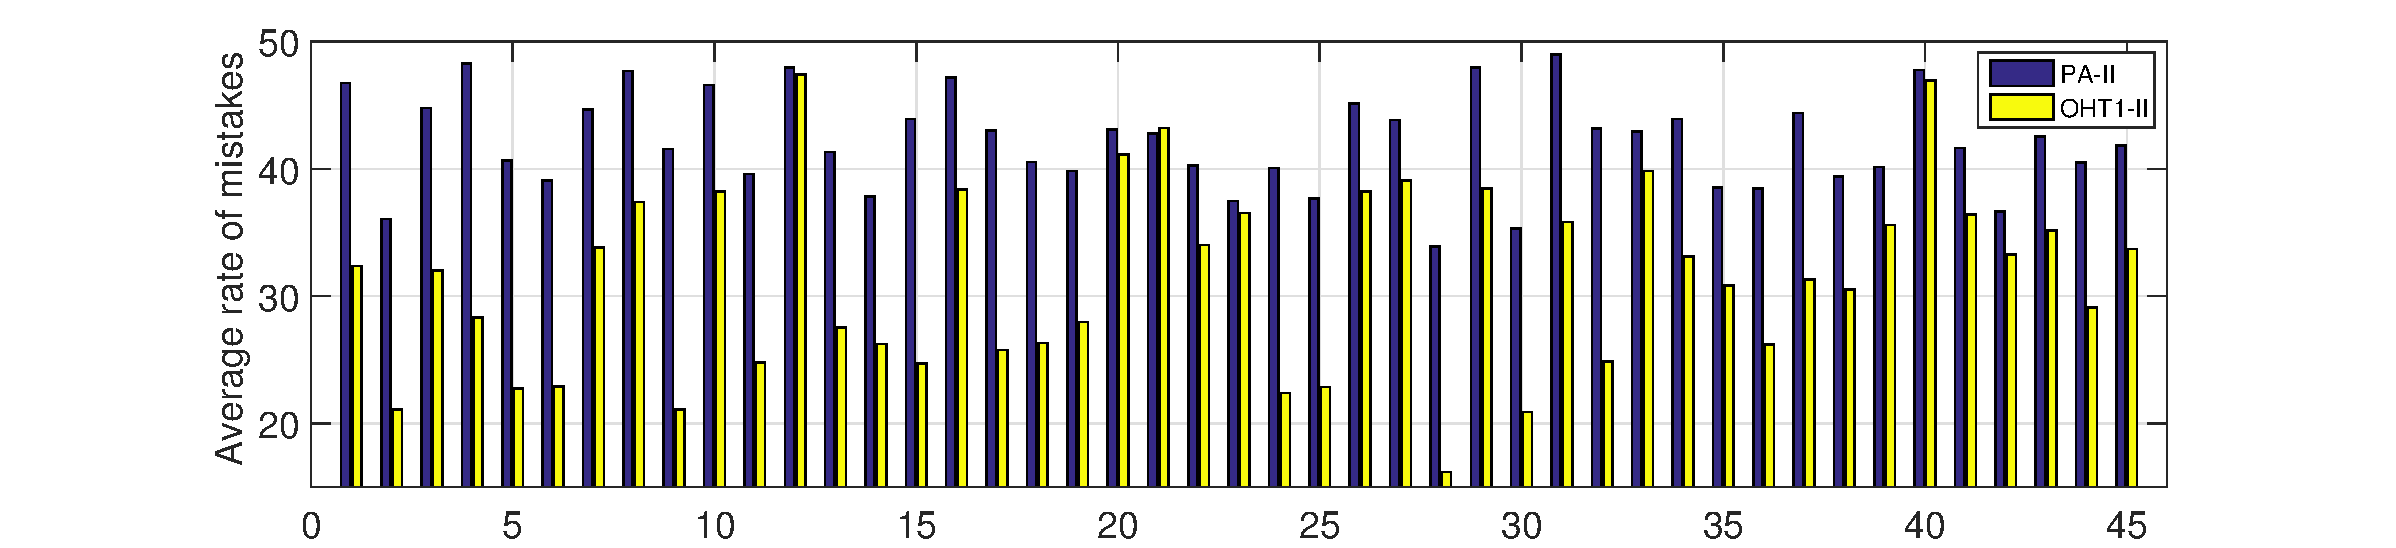
\includegraphics[width=18cm]{12_2.pdf}
  }
  \subfigure[PA-\uppercase\expandafter{\romannumeral2} vs. OHT2-\uppercase\expandafter{\romannumeral2}]
  {
    \label{12}
    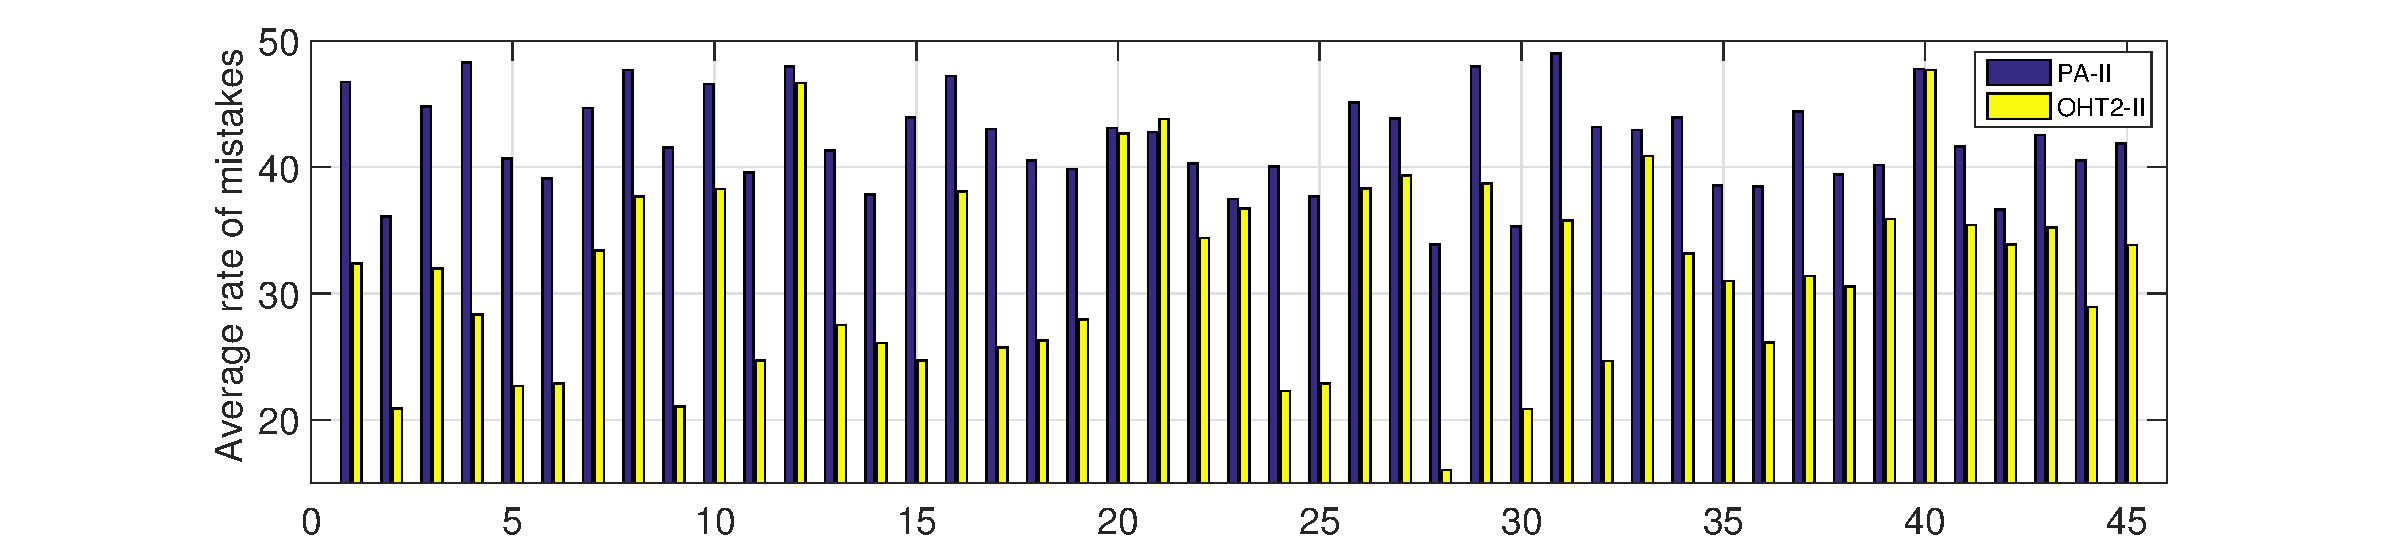
\includegraphics[width=18cm]{22_2.pdf}
  }
  \caption{Average rate of mistakes on all 45 tasks}
  \label{Average rate of mistakes on all 45 tasks}
\end{figure*}

Figure \ref{Average rate of mistakes on all 45 tasks} summarizes the mistake rates of all 45 binary classification tasks in the third set, which compares OHT1-\uppercase\expandafter{\romannumeral2}, OHT2-\uppercase\expandafter{\romannumeral2} and PA-\uppercase\expandafter{\romannumeral2}.
The x-axis of the figure refers to the 45 tasks.
We see that on most tasks, PA-\uppercase\expandafter{\romannumeral2} has the very high mistake rate, which prove the dificulty of image classification task without any auxiliary source information and the necessity of knowledge transfer.
The observation that our proposed OHT methods in general outperform Passive-Aggressive algorithm validates the effectivity of heterogeneous transfer learning.
Similar experimental results are observed in other two sets.
Because of the restricted space, we are not able to report them.
In order to facilitat the description, we denote PA-\uppercase\expandafter{\romannumeral2}, OHT1-\uppercase\expandafter{\romannumeral2} and OHT2-\uppercase\expandafter{\romannumeral2} by PA, OHT1 and OHT2 respectively in the following discussion.

\begin{figure*}[!htb]
\centering
  \subfigure[Task 2]
  {
    \label{task2}
    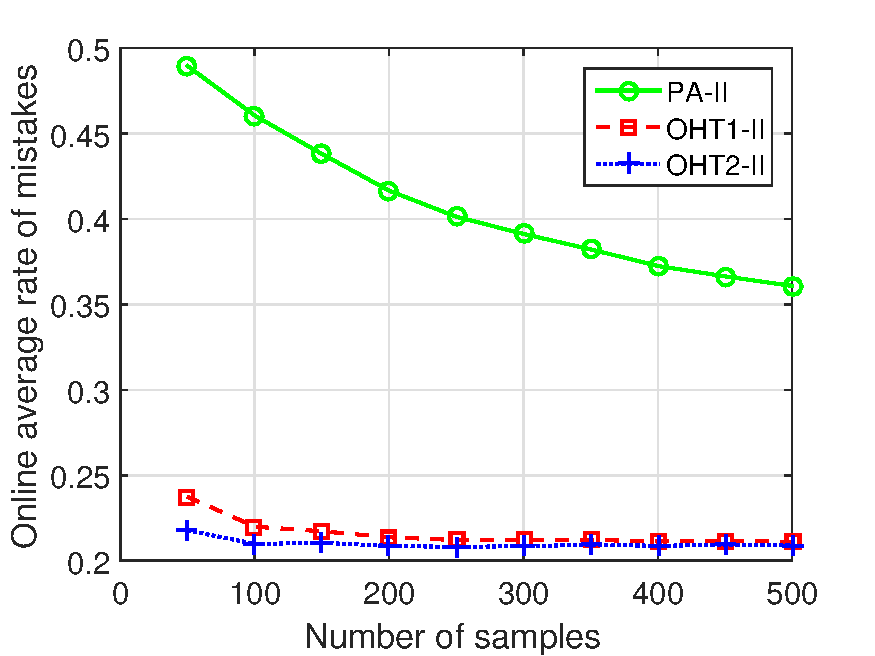
\includegraphics[width=5cm]{task2_2.pdf}
  }
  \subfigure[Task 14]
  {
    \label{task14}
    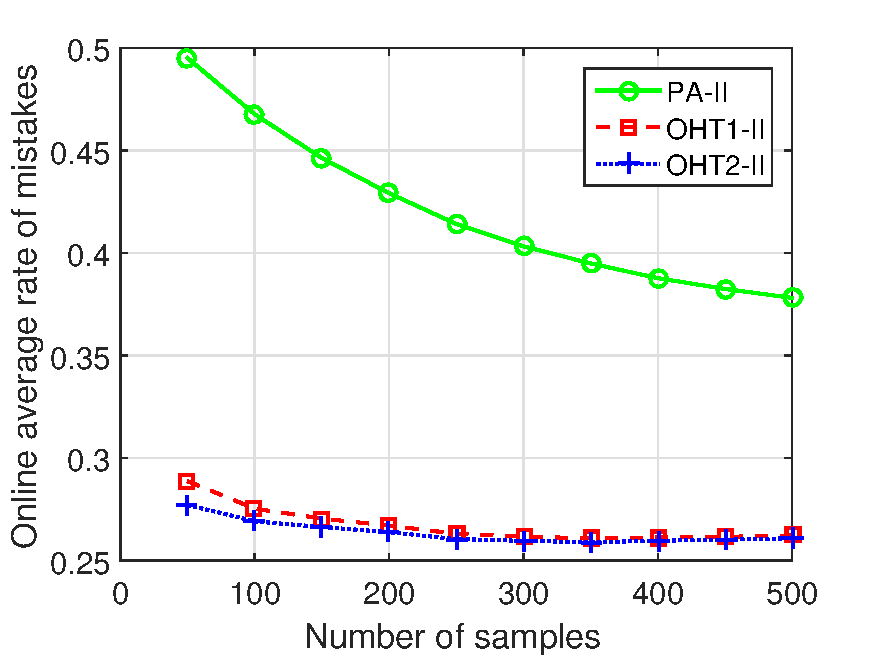
\includegraphics[width=5cm]{task14_2.pdf}
  }
  \subfigure[Task 36]
  {
    \label{task36}
    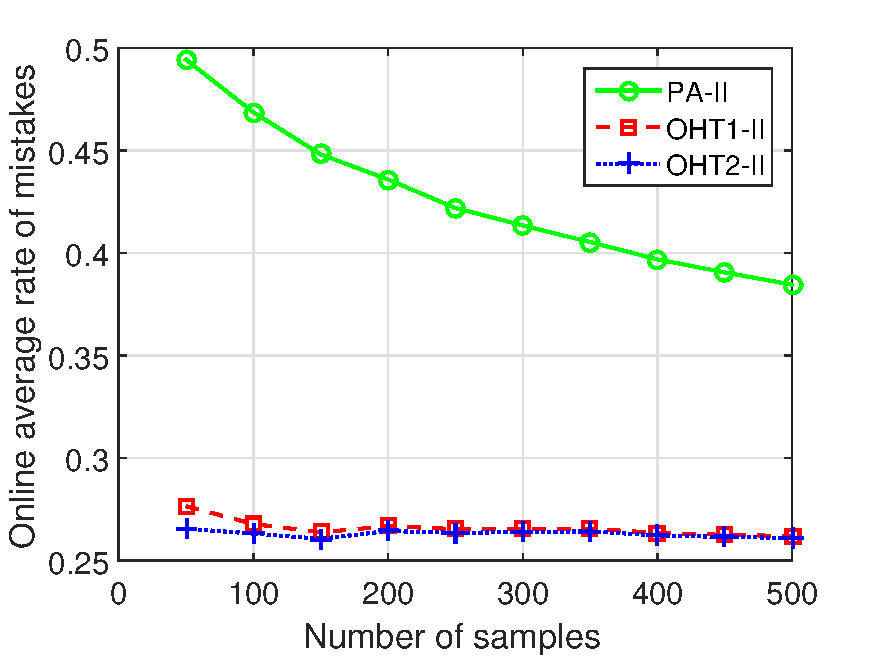
\includegraphics[width=5cm]{task36_2.pdf}
  }
  \\
  \subfigure[Task 7]
  {
    \label{task7}
    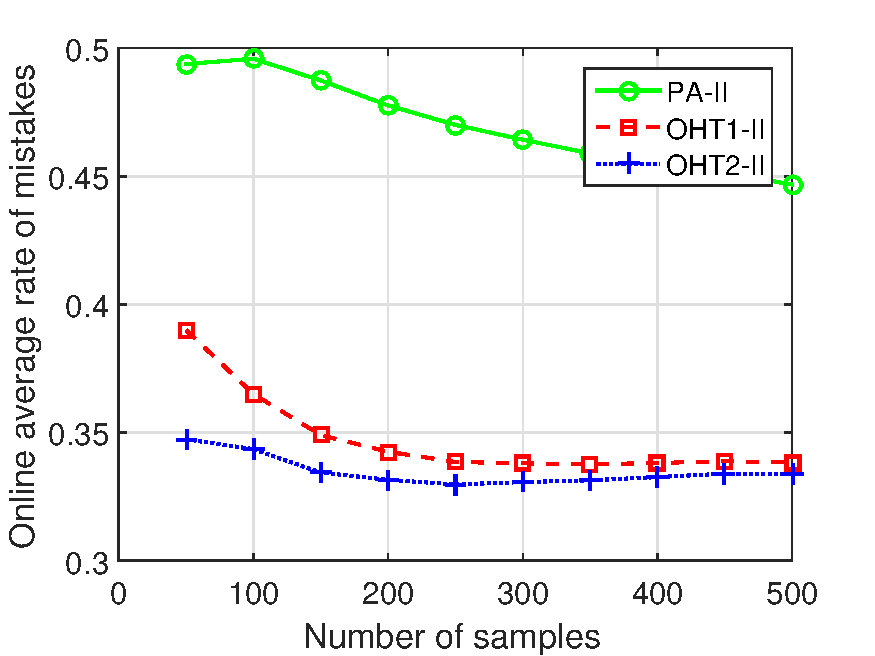
\includegraphics[width=5cm]{task7_2.pdf}
  }
  \subfigure[Task 16]
  {
    \label{task16}
    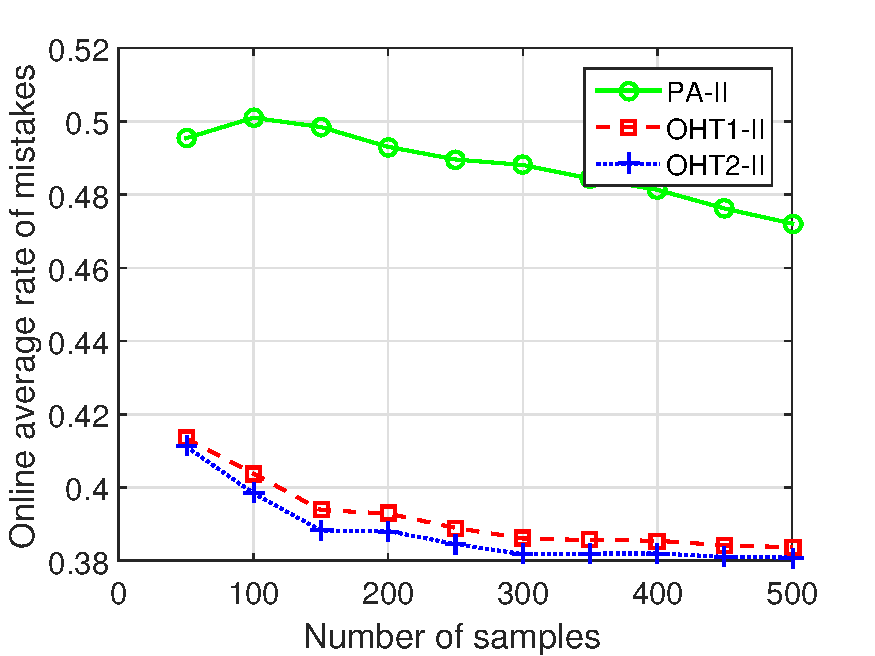
\includegraphics[width=5cm]{task16_2.pdf}
  }
  \subfigure[Task 33]
  {
    \label{task33}
    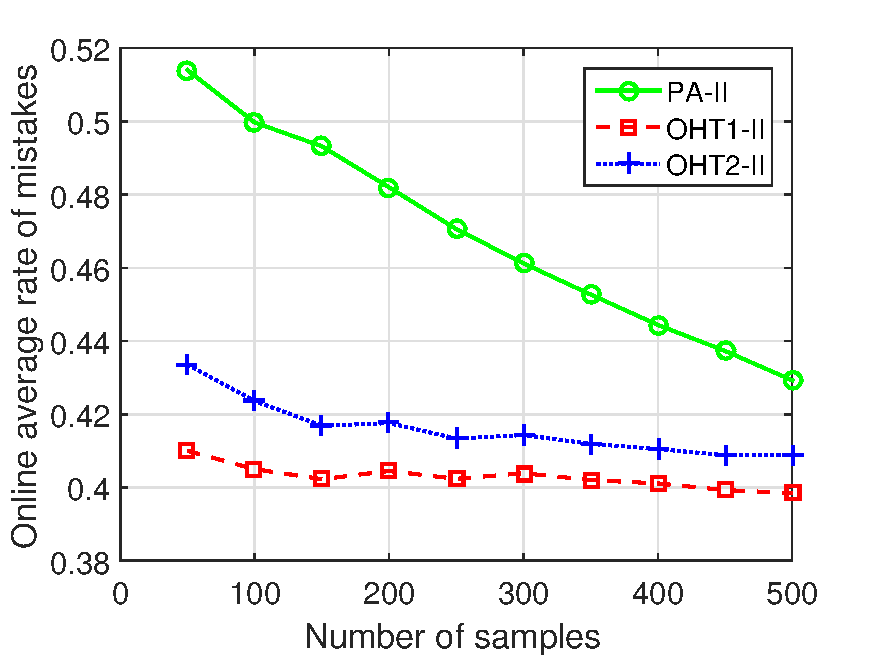
\includegraphics[width=5cm]{task33_2.pdf}
  }
  \caption{Online average rate of mistakes on example tasks}
  \label{Online average rate of mistakes on example tasks}
\end{figure*}

Figure \ref{Online average rate of mistakes on example tasks} illustrates the dynamic process of several representative online learning tasks, respectively.
We observe that OHT algorithms usually achieve better performance at the beginning stage.
On some tasks(e.g., 7, 16 and 33), the online mistake rates of all three algorithms decrease during the period, and OHT methods always obtain better performance than PA algorithm.
These observations verifies that the OHT algorithms indeed transfer useful knowledge from the heterogeneous source domain to the target domain. 

We also analyze the performance difference between PA and two OHT algorithms.
Statistical significance against PA was assessed by paired $t$-test at 0.01 level.
For each task, a win (or loss) is counted when OHT algorithm is significatly better (or worse) than PA algorithm over 100 runs.
Otherwise, a tie is recorded.
The win/tie/loss results is 44/0/1 for competition between OHT1 and PA, and 42/2/1 for competition between  OHT2 and PA.
This result validates that our OHT algorithms is statistically better than PA algorithm.

Besides, we utilize Cohen's $d$ value to measure the improvement of our algorithms.
Generally, $d>0.8$ indicates a large promotion, and $0.2<d<0.8$ indicates a middle promotion.
In our experiments, OHT1 algorithm achieves large improvement on 41 tasks and middle improvement on 3 tasks.
For OHT2 algorithms, the numbers are 40 and 3.
Combining the win/tie/loss results, we see that OHT1 is more stable than OHT2.


\subsection{Parameters and Running time}
% parameter sensitivity
\paragraph{Parameters}
Experiments in paper about online transfer learning illustrated that the performance of online transfer learning algorithms is generally insensitive to the parameter $C$ and $\beta$.
Consequently, we only investigate how different values of parameter $K$ affect the mistake rates of the algorithms.
Figure \ref{average_error} shows the average mistake rates with varied values of parameter $K$ over all 45 tasks.
PA algorithm, whose performance is not related to the parameter $K$, provide a baseline rate of mistakes.
We observe that the performance of the proposed methods consistently outperform PA algorithm, which indicates that nearest neighbors in heterogeneous source domain do provide valuable advice for the classification task.

\begin{figure}[!htb]
\centering
  \subfigure
  {
    \label{average_error}
    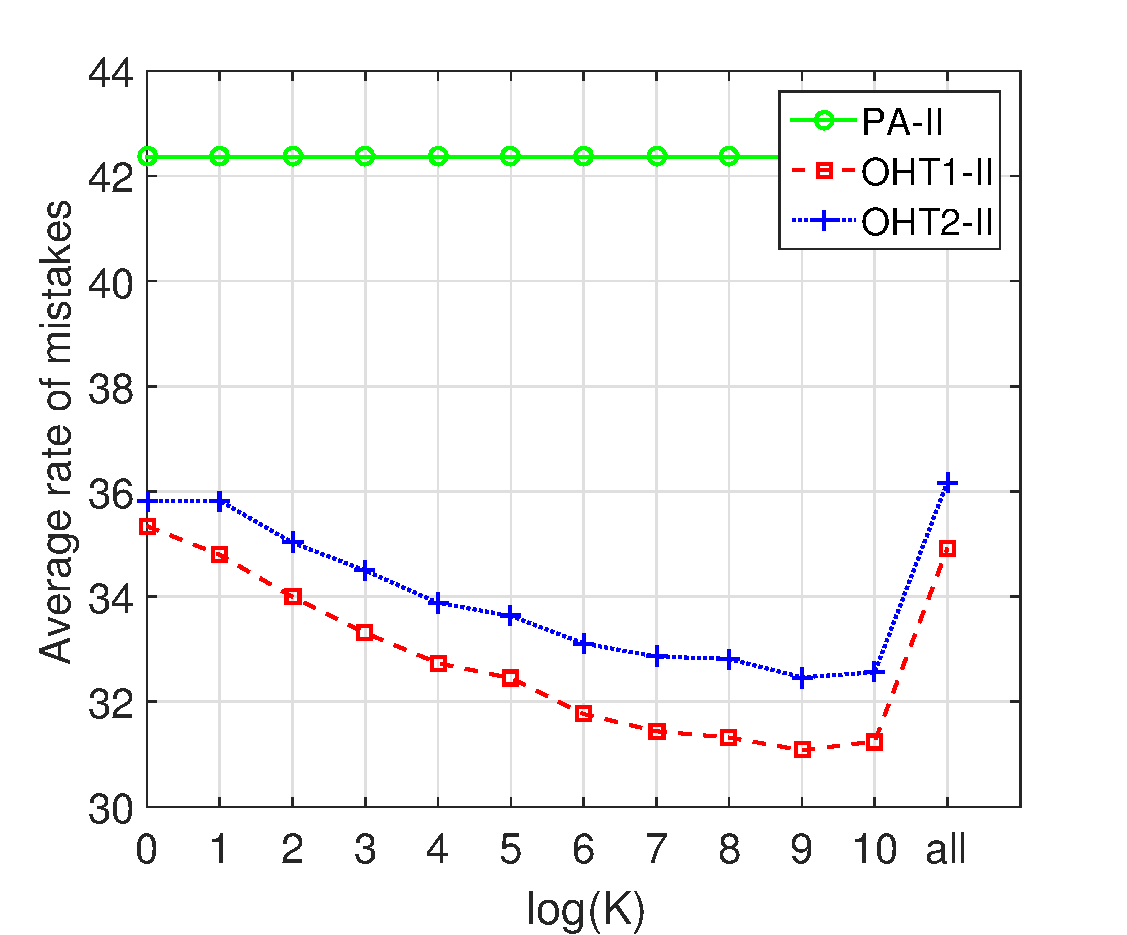
\includegraphics[width=3.9cm]{average_error.pdf}
  }
  \subfigure
  {
    \label{average_time}
    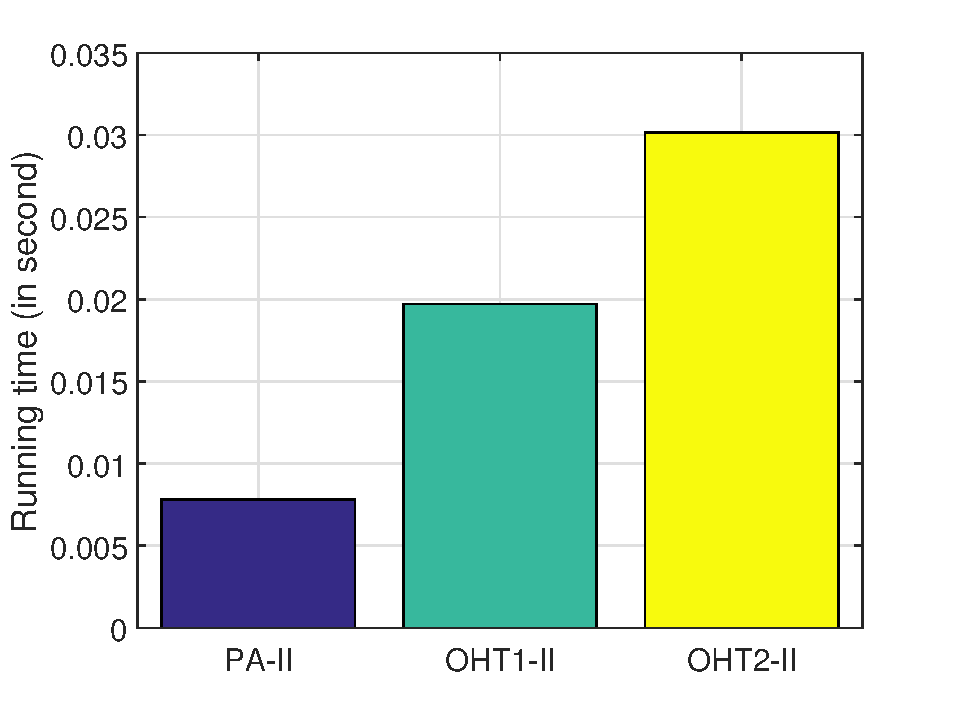
\includegraphics[width=3.9cm]{average_time.pdf}
  }
  \caption{(a) The average rate of mistakes under varying values of $K$. (b) The average running time of different algorithms when all instances in heterogeneous source are considered.}
  \label{average eok}
\end{figure}

% running time
\paragraph{Running time}
All of the algorithms were implemented in Matlab, and all experiments were run in a Linux machine with 3.2 GHz CPU and 3.8 GB memory.
Compared to PA algorithm without exploiting any information from the source domain, OHT algorithms are less efficient.
The main reason of more running time for OHT algorithms is probably the searching process for the nearest neighbors.
We can simply make use of all instances in the heterogeneous source domain to get rid of overhead for searching nearest neighbors.
Figure \ref{average_time} shows the running time of different algorithms when all instances in the heterogeneous source domain are considered.
We obtain generally comparable running time to PA, and at the same time, achieve better performance than PA.

\section{Conclusion}

In this paper, we explore online heterogeneous transfer learning problem, whose objective is to tackle an online classification task on a target domain by leveraging knowledge extracted from a heterogeneous source domain.
We construct a connection across the domains using co-occurrence data, and apply the ensemble strategy to train a classifier based on two hypotheses coming from different domains.
We also offer the theoretical analysis of our algorithms.
Experimental results show that the proposed algorithms significantlly outperform the baseline methods.
In the future, we will consider the application with other types of data, or the scenario which includes more than one source domains.

\bibliographystyle{aaai}
\bibliography{transferlearning,onlinelearning}

\end{document}
